\chapter{Integrating PETSc Linear Solvers into Lighthouse}
\label{addingpetscchap}

Sparse matrices often appear in various fields of science and engineering when solving partial differential equations. Writing PETSc programs to solve sparse linear systems can be very challenging for individuals with little or no programming experience. Since PETSc is one of the most widely used software packages for sparse matrix algebra operations, having Lighthouse to provide PETSc programs to solve them will be highly beneficial to the scientific computing community. What will be even more helpful is to enable Lighthouse to make intelligent suggestions on which Krylov subspace method and preconditioner to apply for solving a particular system of linear equations as quickly as possible. In order to do that, first, we formed a dataset consisting of a large number of real sparse matrices and solved them using various different combinations Krylov subspace methods and preconditioners to record their performances. Then we computed various properties of the matrices to create a set of features. Next, we applied machine learning techniques to train Lighthouse and tested it to check its ability to make good suggestions.

This chapter describes the process of adding the functionalities of PETSc linear solvers to Lighthouse and training it to provide helpful suggestions to the users. Section 4.1 describes various features of PETSc and explains why we chose to integrate PETSc into Lighthouse. Section 4.2 discusses the main use cases. Section 4.3 presents the user interface for using the PETSc functionalities. Section 4.4 explains the matrix properties we extracted and their analysis. Section 4.5 talks about our matrix dataset. Section 4.6 talks about the methods we used for solving the linear systems.  Sections 4.7 discusses the machine learning methods we employed. Section 4.8 concludes the chapter with a discussion on the results.

\section{PETSc}

The Portable, Extensible Toolkit for Scientific Computation (PETSc) is a collection of routines and data structures that provide the building blocks for developing parallel numerical solution of partial differential equations (PDEs) and other related problems in high-performance computing  \cite{petscman}. PETSc is an open source software package written in the C programming language. It is  developed and maintained by Argonne National Laboratory. The development of PETSc began several years ago, and since then it has evolved into a powerful set of tools. It is now the world's most widely used parallel numerical software library for partial differential equations and sparse matrix computations.

PETSc contains a growing collection of parallel linear and nonlinear equation solvers and time integrators that can be employed in application codes written in C, C++, Fortran, Python, and MATLAB. At the time of this writing, the latest version of PETSc is 3.4, released publicly on May 13, 2013. PETSc uses the Message Passing Interface (MPI)  \cite{mpi} standard for all interprocess communication. The following subsections briefly review Krylov subspace methods and preconditioners, describe the structure of PETSc and explain why we chose PETSc.

\subsection{KSP: Krylov subspace methods}
KSP methods are among the most successful methods currently available in numerical linear algebra. These methods are designed for solving nonsingular systems of the form,

\begin{equation}
Ax = b,
\end{equation}

\noindent where \textit{A} is the matrix representation of a linear operator, $b$ is the right-hand-side vector, and $x$ is the solution vector. A Krylov subspace of dimension $r$ is defined by the linear subspace spanned by the images of $b$ under the first $r$ powers of $A$, that is,

\begin{equation}
K_r(A,b) = \mbox{span}\{b, Ab, A^2b, . . . , A^{r-1}b\}.
\end{equation}

\noindent  Modern iterative methods for solving large systems of linear equations avoid matrix-matrix operations. Instead, these methods multiply vectors by the matrix and work with the resulting vectors. Starting with a vector $b$ first $Ab$ is computed, then that vector is multiplied by $A$ to obtain $A^{2}b$ and so on. The algorithms that uses this technique are referred to as Krylov subspace methods.

\subsection{PC: Preconditioners}
In most modern numerical codes for the iterative solution of a linear system, a Krylov subspace method is used in combination with a preconditioner. In numerical linear algebra, a preconditioner $P$ of a matrix $A$ is a matrix such that $P^{-1}A$ has a smaller condition number than $A$, where the condition number is a scalar value associated with the linear equation $Ax = b$ that gives a bound on how inaccurate the solution $x$ will be after approximation.

\subsection{Structure and features of PETSc}
PETSc is made up of a variety of libraries for manipulating different kinds of objects such as vectors, matrices and the operations one would like to perform on the objects. The objects and operations in PETSc were designed and implemented by highly experienced computational scientists with decades of experiences with scientific computation. The following list describes some of the main PETSc modules and their functionalities.

\begin{itemize}
  \item{} Vectors (Vec): This module provide the vector operations required for setting up and solving large-scale linear and nonlinear problems.
  \item{} Matrices (Mat): A large suite of data structures and code for the manipulation of parallel sparse matrices. It includes four different parallel matrix data structures, each appropriate for a different type of problem.
  \item{} Krylov Subspace Methods (KSP): This module provides parallel implementations of many popular Krylov subspace iterative methods. All of the methods are coded and ready to use with any preconditioner and any matrix data structures.
  \item{} Preconditioners (PC): A collection of sequential and parallel preconditioners.
  \item{} Index Sets (IS): For creating and manipulating various types of index sets.
\end{itemize}

\begin{figure}[h!]\label{petscOrganization1}
  \centering
  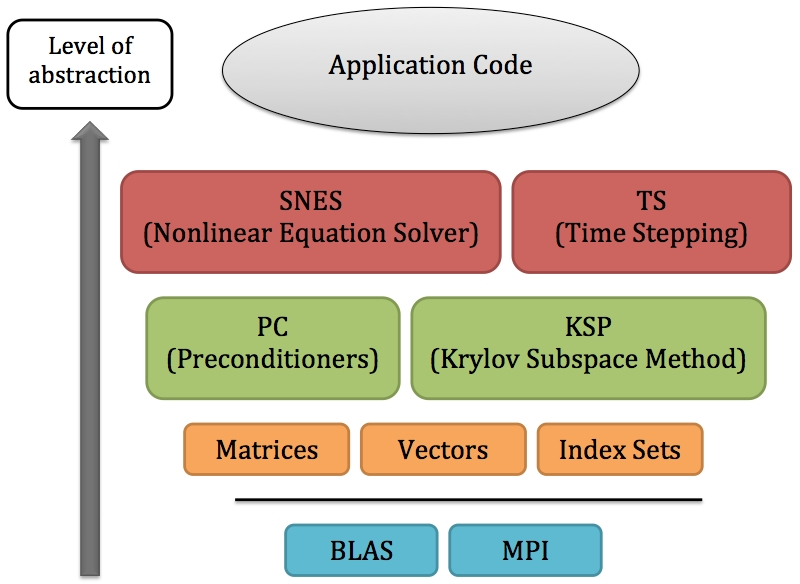
\includegraphics[width=6in]{figs/petscOrganization1}
  \caption[ PETSc libraries]
   {Hierarchical Organization of PETSc libraries.}
\end{figure}

\noindent  The hierarchical infrastructure of PETSc provides a solid foundation for the development of large-scale scientific applications. It also lets the users apply the most appropriate abstraction level for a particular problem and easily customize and extend both algorithms and implementations. It separates the various problems of parallelism from the choice of algorithms. PETSc's hierarchical organization is illustrated in figure 4.1. At the lowest level there are BLAS and MPI libraries. The libraries that provide matrix, vector and index set operations rely on the BLAS and MPI libraries. Next, the PC and KSP libraries use the libraries from the level below them and finally the SNES and TS libraries make use of the PC and KSP libraries. The application code written by a PETSc user is at the highest level of abstraction, meaning the application code simply uses these libraries without having to deal with the underlying details of their implementations.

\subsection{Why we like PETSc} Each of the PETSc modules contains an abstract interface and implementations using specific data structures, allowing PETSc to provide neat and effective codes for the different stages of solving PDEs. PETSc's modular and clean design makes comparing and using different algorithms very easy, which is one of the main reasons we decided to integrate PETSc linear solvers into Lighthouse. We wanted to experiment with various Krylov subspace methods and preconditioners and PETSc provides the perfect environment for such experimentations. PETSc allows executing a program from the command line using a variety of settings. A simple script can be written to solve a particular system using varying number of processes, KSP methods and proconditioners. This particular features has proven to be very useful for our purpose. Moreover,  PETSc's clean and thorough documentation and hundreds of well-commented example codes provide a great environment for learning programming in PETSc.

\paragraph{}
Some of the other popular software packages that offer sparse iterative solvers are SPARSKIT \cite{sparskit}, SLAP \cite{slap}, ITPACK \cite{itpack}, ITSOL \cite{itsol}, ViennaCL \cite{viennacl}, Belos package \cite{belos} by Trilinos \cite{trilinos}. However, none of these packages provide the rich and unique environment for sparse matrix algebra computations that PETSc does.

\section{Primary use cases}

In this section we present the main use cases to show how a user will interact with Lighthouse (the system) in order to have a PETSc program generated. In software engineering, a use case is a list of steps that illustrates how users will perform a task using a software application or a website. It outlines the behavior of a system, from the point of view of a user, as it responds to the user's requests. In the Unified Modeling Language (UML) \cite{uml}, a user who interacts with the system is known as an ``actor''. Preconditions of a use case specify circumstances that must be true before a use case is invoked. Postconditions of a use case list possible situations that the system can be in after the use case is executed. The normal or basic flow of a use case is the flow of actions that is considered normal or usual for the system. Alternate flows are the alternative actions that can be performed. Following are the two main use cases.\\
\\ 
\textbf{Use case: 1}\\
Use case name: Selecting the main task\\
Actors: User\\
Preconditions: The user is at the Lighthouse for PETSc homepage\\
Postconditions: The user is on the web page that handles the task user selected\\
Normal Flow:
\begin{enumerate}
  \item Lighthouse provides the user with a list of tasks that they can choose from. 
  \item The user selects the task they would like to perform. 
  \item User submits the form by clicking the submit button. 
  \item Lighthouse presents the appropriate page to the user based on the task they chose.\\
\end{enumerate}

\noindent \textbf{Use case: 2}\\
Use Case Name: Solving a linear system\\
Actors: User\\
Preconditions: User is at the ‘Solve a Sparse Linear System’ page\\
Postconditions: User has the archive file that contains a PETSc program and necessary instructions for solving their system of linear equations.\\
\textbf{Normal Flow:}
\begin{enumerate}
  \item Lighthouse asks the user if they want to upload their matrix. 
  \item User chooses to upload their matrix. 
  \item Lighthouse provides the user with a file browser for selecting the matrix file. 
  \item User selects the matrix file. 
  \item Lighthouse asks the user if they want a sequential solution or a parallel solution. 
  \item User selects the type of solution they want. 
  \item User submits the form. 
  \item Lighthouse generates a PETSc program in C programming language, a makefile, a text file containing the command line options and a readme file. 
  \item Lighthouse then creates an archive file containing the files generated in step 8. 
  \item Lighthouse provides the user with a download link of the archive file.
  \item User downloads the archive file.
  \item Lighthouse deletes any file from the server that the user had uploaded.
\end{enumerate}
\textbf{Alternate Flows:} \\ 
2A1: User does not want to upload their matrix. 
\begin{enumerate}
  \item User chooses not to upload their matrix.
  \item Lighthouse asks the user if they would like to download a PETSc program to compute the matrix properties themselves and upload the output of the program or download a general PETSc program for solving a sparse system of linear equations. 
  \item User chooses to download the matrix property computation program.
  \item Lighthouse provides a link to an archive file containing the matrix property computation program and other necessary files.
  \item User downloads the file.
  \item User computes the matrix properties using the downloaded program.
  \item User returns to Lighthouse and selects the option for uploading the matrix property file.
  \item Lighthouse provides the user with a file browser for selecting the matrix property file. 
  \item User selects the matrix property file.
  \item Lighthouse asks the user if they want a sequential solution or a parallel solution. 
  \item User selects the type of solution they want. 
  \item User submits the form. 
  \item The use case continues from step 8 of the normal flow.
\end{enumerate}
2A1.2A: User chooses to download the general PETSc program for solving a sparse system of linear equations.
\begin{enumerate}
  \item User submits the form. 
  \item The use case continues from step 8 of the normal flow.
\end{enumerate}

\noindent These uses cases provide the foundation for building an interactive system that will enable users to have PETSc programs generated for solving their sparse linear systems.

\section{User interface}
In this section, we discuss the web user interface through which users interact with the system. It is built using the same set of tools that we used for developing the LAPACK and BTO user interfaces of Lighthouse discussed in chapter 3. The user interface is presented using the screen-shots taken from the Lighthouse for PETSc website.

\subsection{Normal flow}
Figure 4.2 shows the Lighthouse for PETSc homepage. On the right part of the homepage, in the Instructions tab, Lighthouse provides the user with information about what this website does followed by instructions on how to use the website. On the left part, in the PETSc Simple Search tab, Lighthouse asks the user which task they would like to perform and provides the options. Initially, the other tabs labeled PETSc Code tab (appears next to the Instructions tab), Command-line Options and Makefile tabs (appear under the Instructions tab) do not have any contents but they become available after Lighthouse prepares the files for the user.

\begin{figure}[H]\label{petscui1}
  \centering
  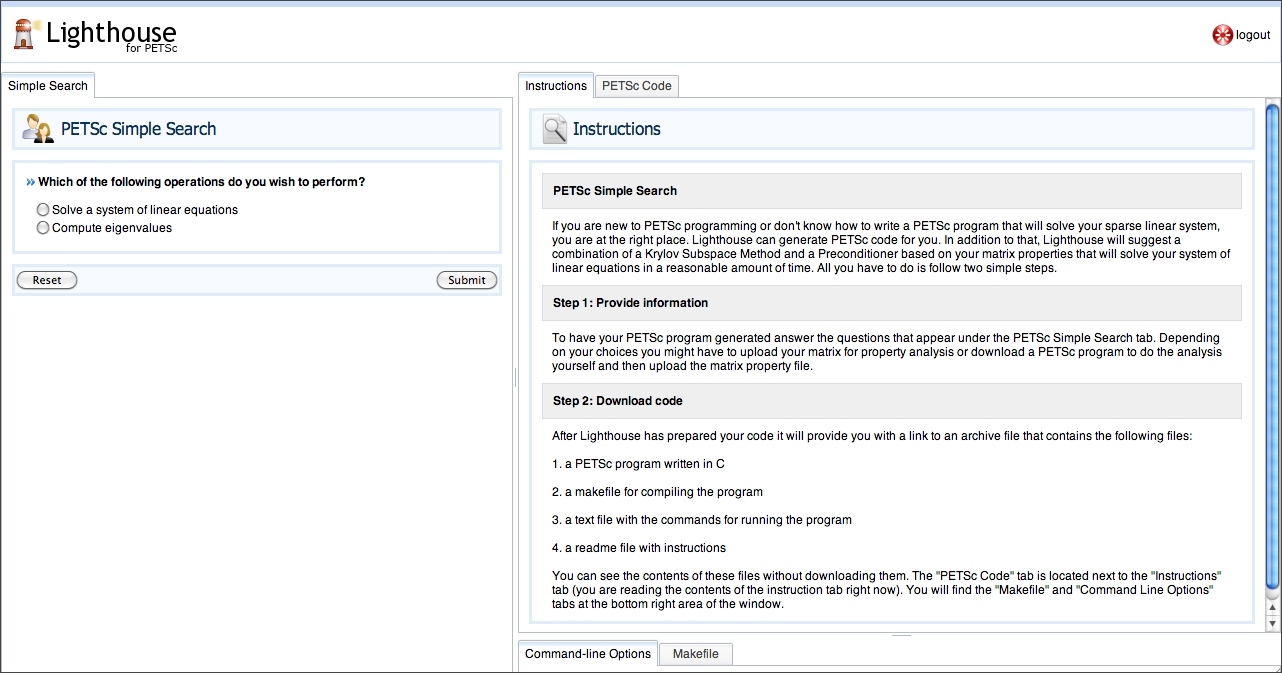
\includegraphics[width=6.5in]{figs/petsc_1}
  \caption[Lighthouse for PETSc homepage.]
   {Lighthouse for PETSc homepage.}
\end{figure}

\noindent Once the user has selected the task `Solve a system of linear equations' and submits the form, Lighthouse asks the user whether they want to upload their matrix (shown in Figure 4.3). If the user chooses to upload their matrix, as shown in Figure 4.4, Lighthouse provides a file picker for the user to select their matrix file. \\

\begin{figure}[H]\label{petscui2}
  \centering
  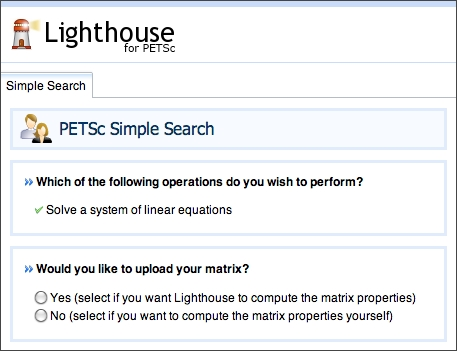
\includegraphics[width=4.5in]{figs/petsc_2}
  \caption[Matrix upload options.]
   {Matrix upload options.}
\end{figure} 

\noindent After the user selects a matrix file, Lighthouse asks the user whether they want a sequential or parallel solution (Figure 4.5). Once the user selects the type of solution they would like to have, Lighthouse asks the user to submit the form (Figure 4.6). After the user submits the form, Lighthouse tells the user that they can download their program (Figure 4.7). At this stage, the code, makefile for compiling the code and commands for running the program can be viewed in their respective tabs before downloading them.

\begin{figure}[H]\label{petscui3}
  \centering
  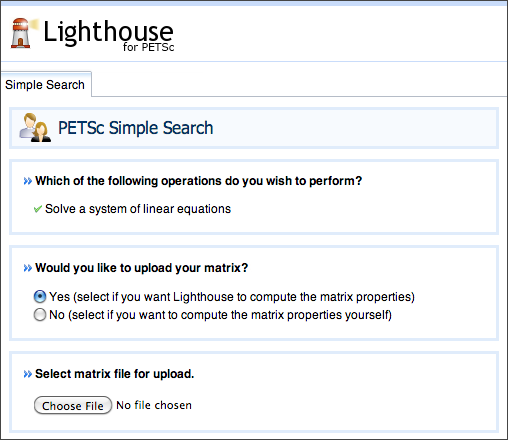
\includegraphics[width=3.85in]{figs/petsc_3}
  \caption[Selecting a matrix file.]
   {Selecting a matrix file.}
\end{figure}

\begin{figure}[H]\label{petscui4}
  \centering
  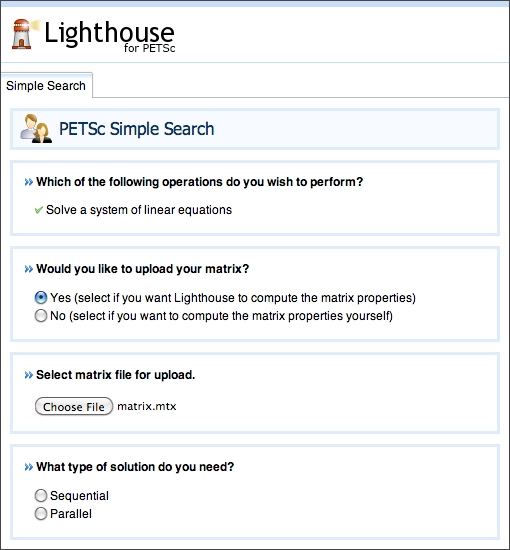
\includegraphics[width=3.85in]{figs/petsc_4}
  \caption[Options for solution type.]
   {Options for solution type.}
\end{figure}

\begin{figure}[H]\label{petscui5}
  \centering
  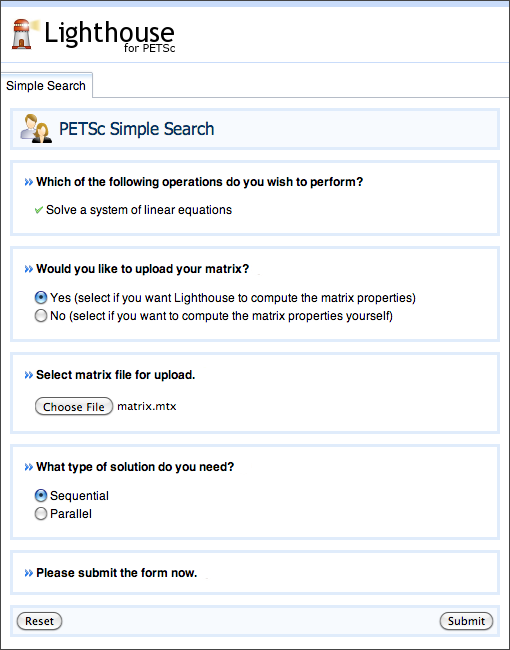
\includegraphics[width=4in]{figs/petsc_5}
  \caption[Submitting the form.]
   {Submitting the form.}
\end{figure}

\begin{figure}[H]\label{petscui7}
  \centering
  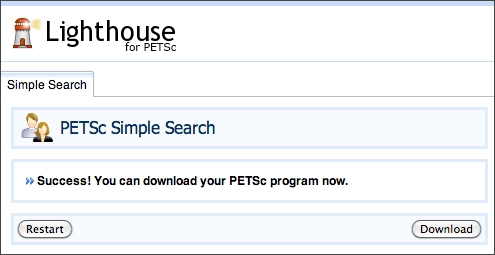
\includegraphics[width=4in]{figs/petsc_7}
  \caption[Downloading the PETSc program.]
   {Downloading the PETSc program.}
\end{figure}

\subsection{Alternate Flow}
If the user chooses to not to upload their matrix, Lighthouse provides the following three options to the user (Figure 4.8).\\
\hspace*{1em} 1. Download a PETSc program for computing matrix properties\\
\hspace*{1em} 2. Download a general PETSc program for solving a linear system\\
\hspace*{1em} 3. Upload matrix properties computed using our program

\begin{figure}[h!]\label{petscui6}
  \centering
  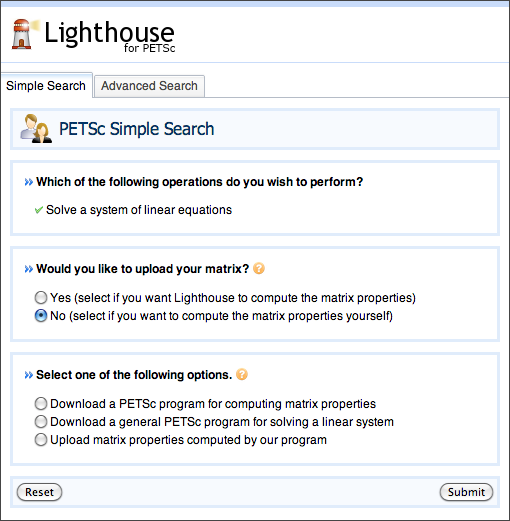
\includegraphics[width=4.5in]{figs/petsc_6}
  \caption[Options for users who choose not to upload their matrix.]
   {Options for users who choose not to upload their matrix.}
\end{figure}

\noindent If the user chooses to download the PETSc program for computing matrix properties and submits the form, they are provided with an archive file containing the matrix property computation program and other necessary files. If the user decides to download a general PETSc program for solving a linear system, Lighthouse gives them a PETSc program for solving a linear system and other necessary files but does not suggest any specific Krylov subspace method or preconditioner. This option is for the users who know what Krylov method and preconditioner they want to use or experiment with.

\begin{figure}[H]\label{petscui8}
  \centering
  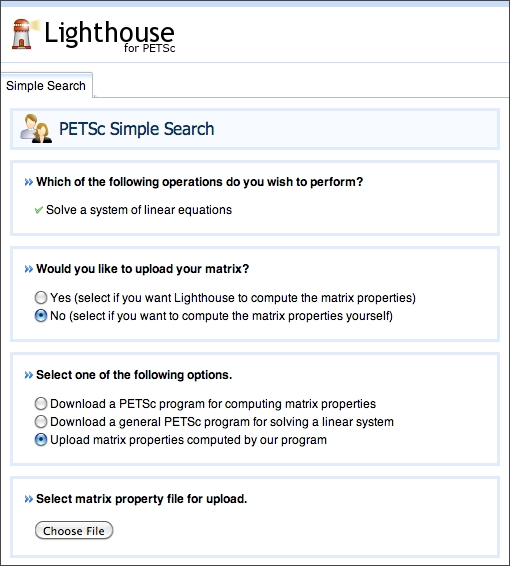
\includegraphics[width=4.5in]{figs/petsc_8}
  \caption[Uploading matrix property file.]
   {Uploading matrix property file.}
\end{figure}

\noindent If the user selects the option for uploading a matrix property file that they prepared using the first option, Lighthouse lets the user select the file using a file picker (Figure 4.9). 

\begin{figure}[H]\label{petscui9}
  \centering
  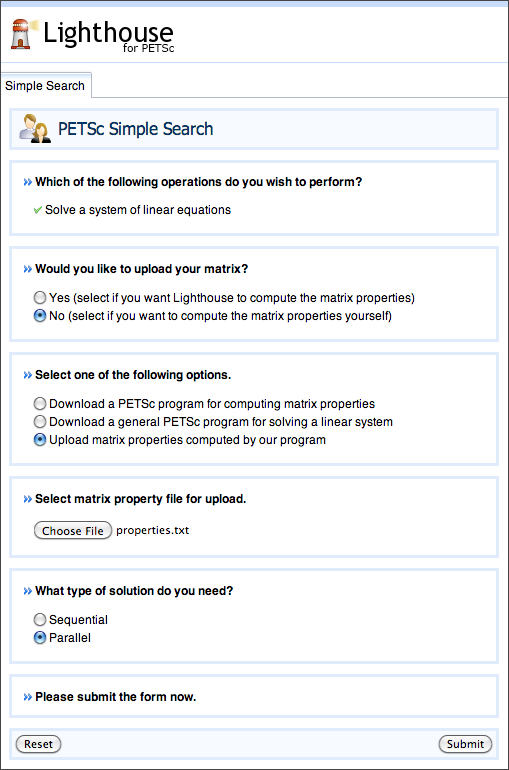
\includegraphics[width=4.5in]{figs/petsc_9}
  \caption[Submitting the form in alternate flow.]
   {Submitting the form in alternate flow.}
\end{figure}

\noindent Once they select the matrix property file, Lighthouse asks them whether they want a sequential or a parallel solution. After the user selects their desired option, Lighthouse asks them to submit the form (Figure 4.10). After the user submits the form, they are provided with an archive file that includes the program and other required files to run the program.

\section{Matrix properties}

We computed thirty properties for each of the matrices in our dataset. These properties play a very crucial role in building our system. We use these properties to form our feature set. In machine learning, a feature specifies a quantitative value of a property of an object. For example, row is an property of a matrix and the number of rows of a matrix is the row feature of that matrix. In this section, we explain the properties we computed. Consider the following $m \times m$ matrix $A$.

\begin{center}
  $A_{m,m} =
 \begin{pmatrix}
  a_{1,1} & a_{1,2} & \cdots & a_{1,m} \\
  a_{2,1} & a_{2,2} & \cdots & a_{2,m} \\
  \vdots  & \vdots  & \ddots & \vdots  \\
  a_{m,1} & a_{m,2} & \cdots & a_{m,m}
 \end{pmatrix}$
\end{center}

\noindent Following is a list of all the properties of $A$ that we compute. 

\begin{enumerate}
\item \textbf{Dimension:} The number of rows and columns of square matrix $A$.
\item \textbf{Nonzeros:} The total number of nonzero entries, that is, the number of entries in $A$ for which $a_{i,j} \neq 0$ is true, where $i$ and $j$ are positive integers and $1 \leq i \leq m$ and $1 \leq j \leq m$.
\item \textbf{Max. nonzeros per row:} The maximum number of nonzero entries in a row of $A$.
\item \textbf{Min. nonzeros per row:} The minimum number of nonzero entries in a row of $A$.
\item \textbf{Avg. nonzeros per row:} The average number of nonzero entries in a row of $A$. 
\item \textbf{Dummy rows:} The number of rows of $A$ with only one nonzero entry.
\item \textbf{Dummy rows kind:} The dummy rows kind of $A$ can be one of the following three. First kind, every dummy row of $A$ has entry 1 at the main diagonal position. Second kind, every dummy row of $A$ has a nonzero entry at the main diagonal position but it is not always 1. Third kind, the nonzero entry is not on the diagonal.
\item \textbf{Hard numeric value symmetry:} If $A$ is equal to its transpose, that is, $A=A^{T}$, then the value of this property is 1. Otherwise, it is 0.
\item \textbf{Hard nonzero pattern symmetry:} If $A$ has the same nonzero pattern as its transpose $A^{T}$, that is, for every nonzero entry $a_{i,j}$ of $A$, $A^{T}$ has a nonzero entry $a_{i,j}$, then the value of this property is 1. Otherwise, it is 0.
\item \textbf{Soft numeric value symmetry:} The soft numeric value symmetry $v$ of $A$ is, \\ $v=1-(\frac{1}{2}\sum_{i=1}^{m}\sum_{j=1}^{m}|s_{i,j}| / \sum_{i=1}^{m}\sum_{j=1}^{m}|a_{i,j}|)$, where $S = (s_{i,j})$ is $\frac{1}{2}(A - A^{T})$, the antisymmetric part of $A$.
\item \textbf{Soft nonzero pattern symmetry:} The ratio of the number of nonzero entries $a_{i,j}$ in $A$, for which, there exist no entry $a_{j,i}$ in $A$, to the total number of nonzero entries in $A$.
\item \textbf{Trace:} The sum of all the diagonal entries of $A$. The trace of $A$ is $\sum_{i=1}^{m} a_{i,i}$.
\item \textbf{Absolute trace:} The sum of the absolute values of all the diagonal entries of $A$. The absolute trace of $A$ is $\sum_{i=1}^{m} |a_{i,i}|$.
\item \textbf{One norm:} The maximum absolute column sum of $A$. More precisely, the one norm of $A$ is $\max\limits_{\substack{1 \leq j \leq m}}(\sum_{i=1}^{m} |a_{i,j}|)$.

\item \textbf{Infinity norm:} The maximum absolute row sum of $A$. The infinity norm of $A$ is $\max\limits_{\substack{1 \leq i \leq m}}(\sum_{j=1}^{m} |a_{i,j}|)$.
\item \textbf{Frobenius norm:} The square root of the sum of all the entries of $A$ squared. The Frobineus norm of $A$ is $\sqrt{\sum_{i=1}^{m}\sum_{j=1}^{m} a_{i,j}^2}$.
\item \textbf{Symmetric infinity norm:} The infinity norm of the symmetric part of $A$. The symmetric part of $A$ is $\frac{1}{2}(A + A^{T})$.
\item \textbf{Symmetric Frobenius norm:} The Frobenius norm of the symmetric part of $A$.
\item \textbf{Antisymmetric infinity norm:} The infinity norm of the antisymmetric part of $A$.
\item \textbf{Antisymmetric Frobenius norm:} The Frobenius norm of the antisymmetric part of $A$.
\item \textbf{Row diagonal dominance:}
This property is 0, if, for any row $i$ of $A$, the absolute value of the diagonal entry in that row is smaller than the sum of the absolute values of the non-diagonal entries. That is,
$|a_{i,i}| < \sum_{j \neq i} |a_{i,j}|$  for all $j$.\\
This property is 1, if $|a_{i,i}| \geq \sum_{j \neq i} |a_{i,j}|$  for all $j$.\\
This property is 2, if $|a_{i,i}| > \sum_{j \neq i} |a_{i,j}|$  for all $j$.
\item \textbf{Column diagonal dominance:}
This property is 0, if, for any column $j$ of $A$, the absolute value of the diagonal entry in that column is smaller than the sum of the absolute values of the non-diagonal entries. That is,
$|a_{j,j}| < \sum_{i \neq j} |a_{i,j}|$  for all $i$.\\
This property is 1, if $|a_{j,j}| \geq \sum_{i \neq j} |a_{i,j}|$  for all $i$.\\
This property is 2, if $|a_{j,j}| > \sum_{i \neq j} |a_{i,j}|$  for all $i$.
\item \textbf{Max. row variance:} The maximum row variance of $A$. The row variance of any row $i$ is $\frac{1}{m}\sum_{j=1}^{m}(a_{i,j} - \mu)^{2}$, where $\mu = \frac{1}{m}\sum_{j=1}^{m} a_{i,j}$.
\item \textbf{Max. column variance:} The maximum column variance of $A$. The column variance of any column $j$ is $\frac{1}{m}\sum_{i=1}^{m}(a_{i,j} - \mu)^{2}$, where $\mu = \frac{1}{m}\sum_{i=1}^{m} a_{i,j}$.
\item \textbf{Diagonal average:} The arithmetic mean of the absolute values of the diagonal entries of $A$. More precisely, diagonal average of $A$ is $\frac{1}{m}\sum_{i=1}^{m} |a_{i,i}|$.
\item \textbf{Diagonal variance:} The variance of the diagonal entries of $A$, that is, $\frac{1}{m}\sum_{i=j=1}^{m}(a_{i,j} - \mu)^{2}$, where $\mu = \frac{1}{m}\sum_{i=1}^{m} a_{i,i}$.
\item \textbf{Diagonal sign:} This property indicates the diagonal sign pattern. Diagonal sign of $A$ is -2 if all diagonal entries of $A$ are negative, -1 if all are nonpositive, 0 if all are zeros, 1 if all are nonnegative, 2 if all are positive, 3 if some are negative and some or none are zero and some are positive.
\item \textbf{Diagonal nonzeros:} The number of nonzero entries in the diagonal of $A$.
\item \textbf{Lower bandwidth:} The smallest number $p$ such that any entry $a_{i,j} = 0$ when $i > j + p$.
\item \textbf{Upper bandwidth:} The smallest number $p$ such that any entry $a_{i,j} = 0$ when $i < j - p$.

\end{enumerate}

\subsection{Principal component analysis of the matrix properties}
Principal Component Analysis (PCA) \cite{smith} is a statistical technique for identifying patterns in data and representing data in a form that highlights the similarities and differences in the data. The patterns found in the data can be used for compressing the data. Performing PCA on a set of data involves adjusting the data set is so that its mean is zero, then computing the covariance matrix of the data set and then finding the eigenvalues and eigenvectors of the covariance matrix. Finally, the eigenvectors are sorted from highest to lowest based on their corresponding eigenvalues. The eigenvector with the highest eigenvalue is the first principal component of the data set. The largest values in the first principal component indicates that the corresponding variables or dimensions account for the highest variance in the data set. Principal components with lower eigenvalues indicate which variables do not provide much information about the variance of the data set.

For the purpose of PCA, we created a data set containing 860 data points where each data point is a 30-dimensional vector. Each vector represents a matrix and the entries in the vector correspond to the properties of the matrix. Then using Matlab's Statistics toolbox, we performed PCA to find out which of the thirty properties account for the most variability in the data. Figure 4.11 provides a bar plot of the eigenvalues of the principal components sorted from highest to lowest based on their eigenvalues. Figure 4.12 shows the first principal component and it tells us that the row, column and diagonal variances account for the most variance in the data. Figure 4.13, 4.14 and 4.15 show the second, third and fourth principal components respectively and indicate how much information various matrix features provide.

\begin{figure}[H]\label{eigenvalues}
  \centering
  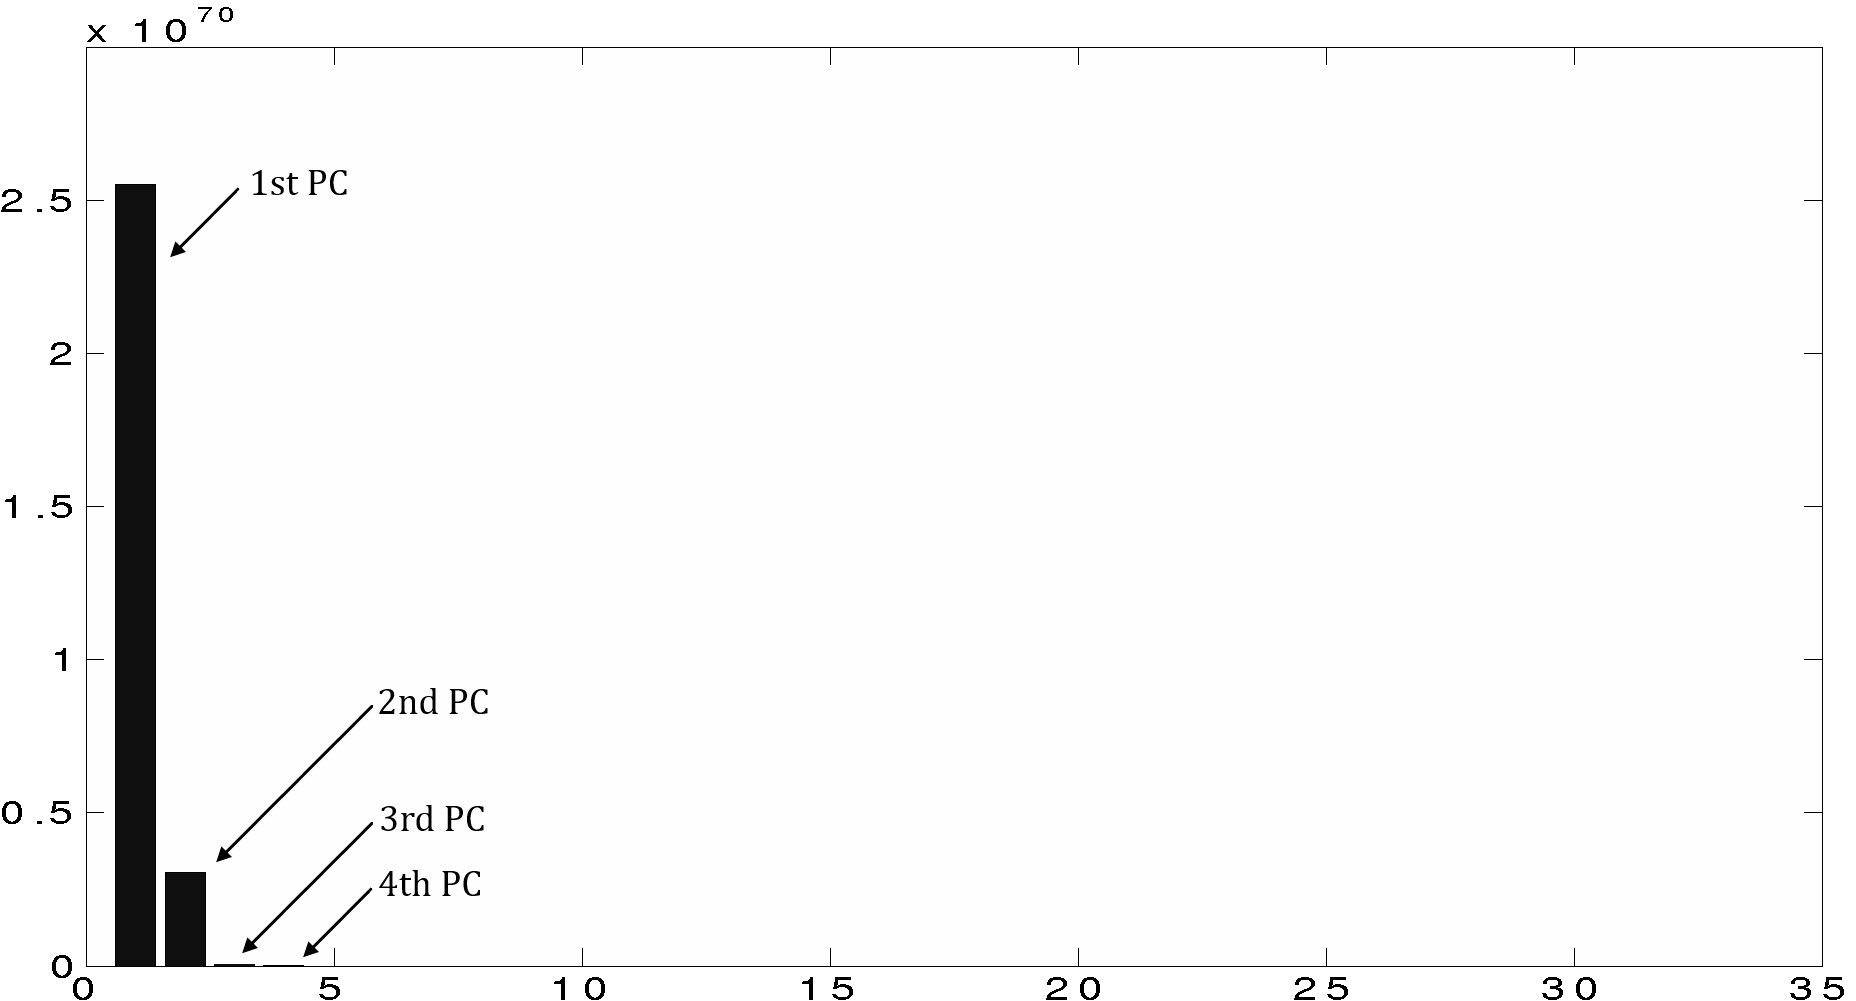
\includegraphics[width=6in]{figs/eigenvalues}
  \caption[Eigenvalues of the principal components.]
   {Eigenvalues of the principal components.}
\end{figure}

\begin{figure}[H]\label{pc_1}
  \centering
  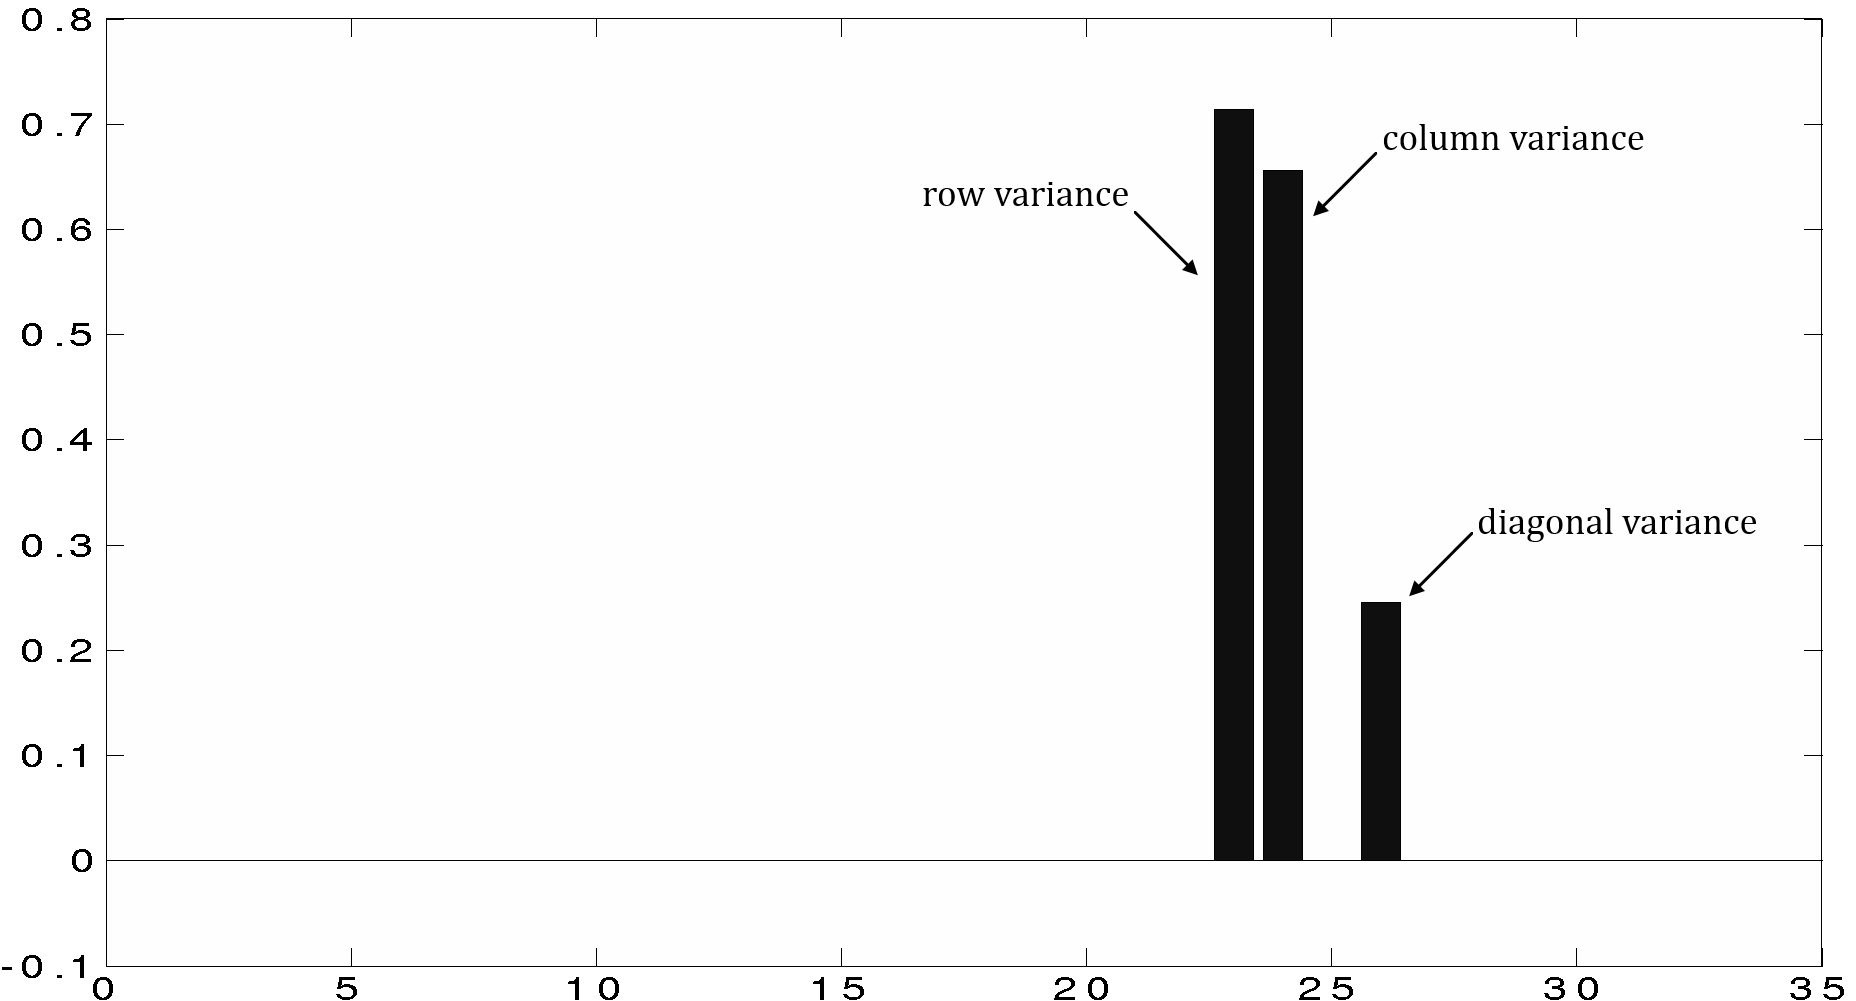
\includegraphics[width=6in]{figs/pc_1}
  \caption[First principal component.]
   {First principal component.}
\end{figure}

\begin{figure}[H]\label{pc_2}
  \centering
  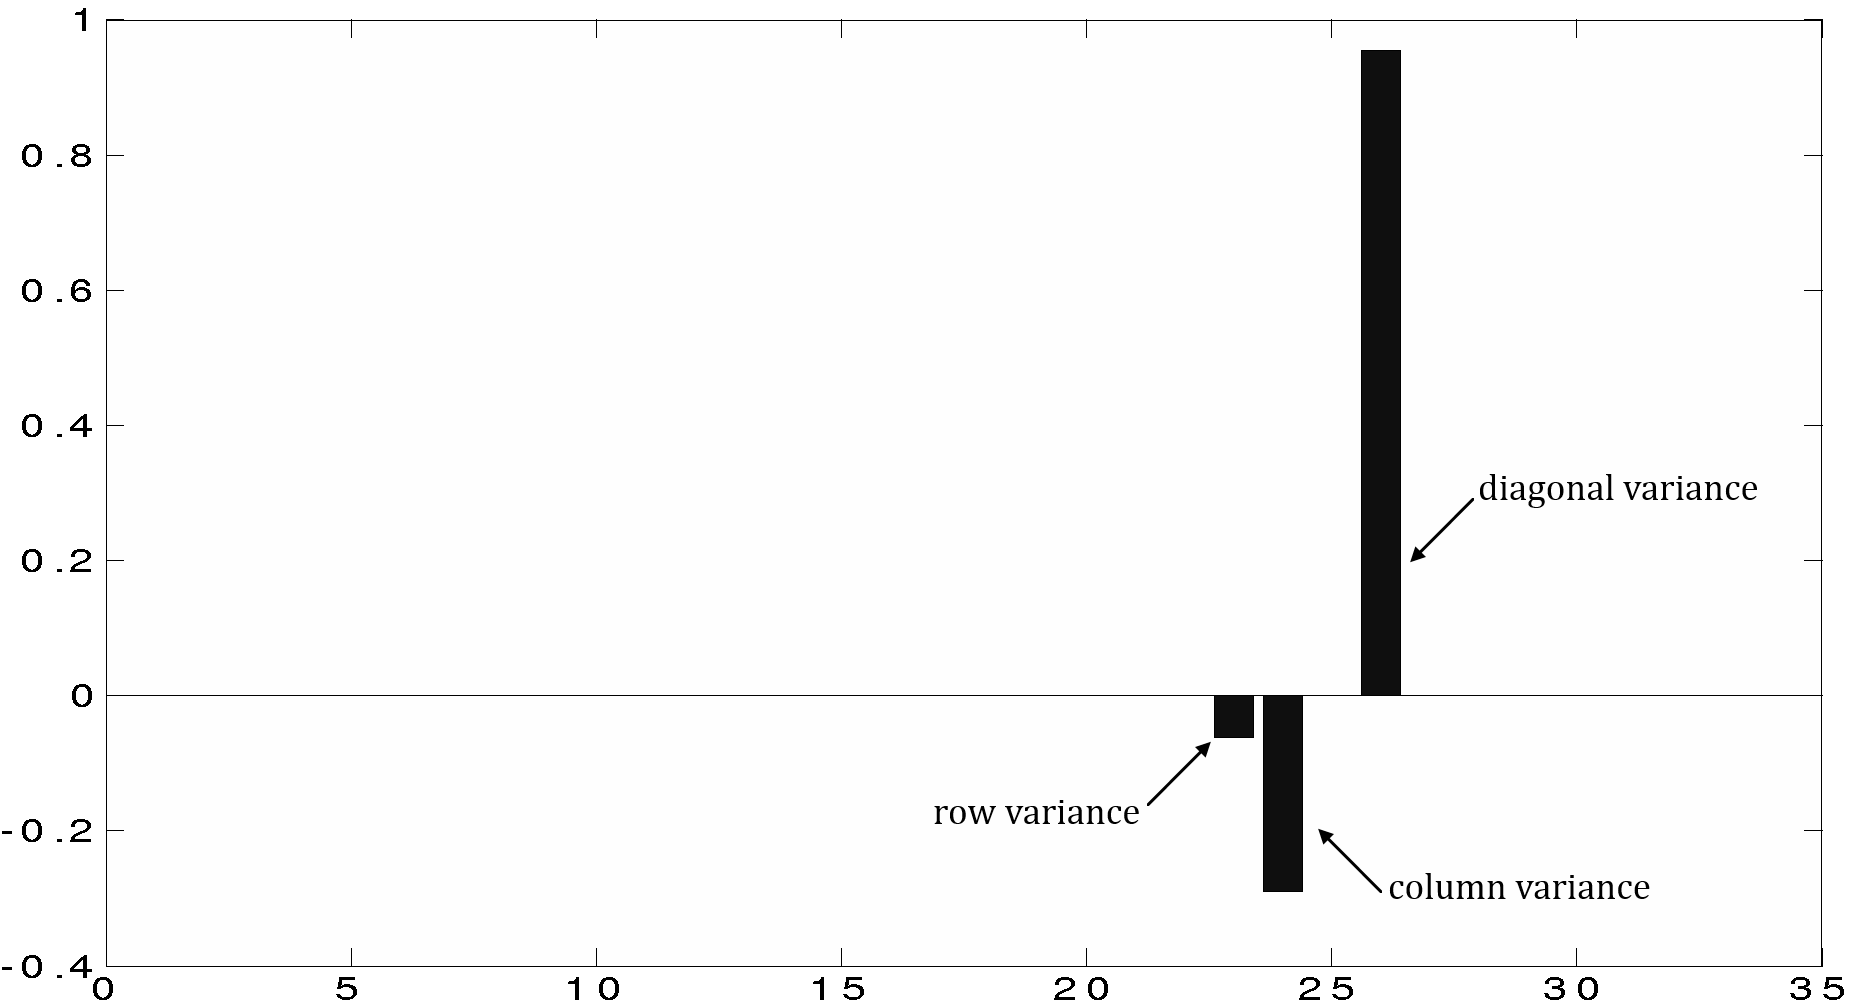
\includegraphics[width=6in]{figs/pc_2}
  \caption[Second principal component.]
   {Second principal component.}
\end{figure}

\begin{figure}[H]\label{pc_3}
  \centering
  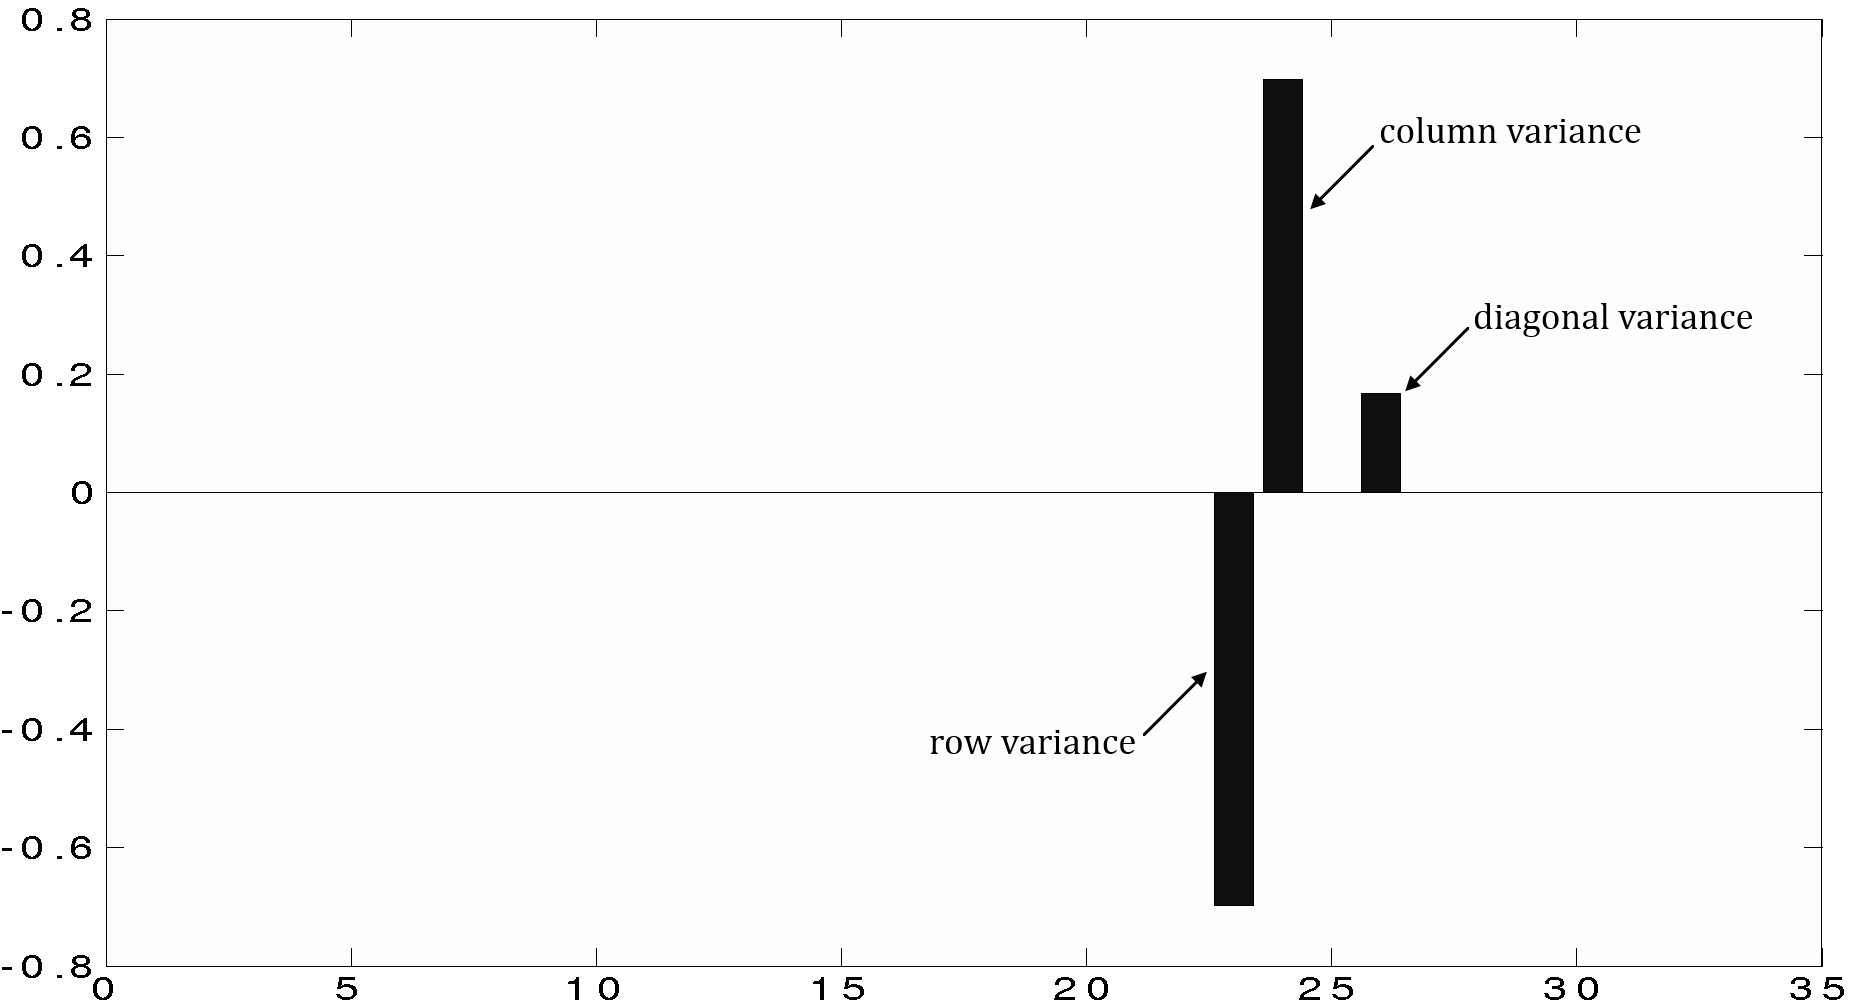
\includegraphics[width=6in]{figs/pc_3}
  \caption[Third principal component.]
   {Third principal component.}
\end{figure}

\begin{figure}[H]\label{pc_4l}
  \centering
  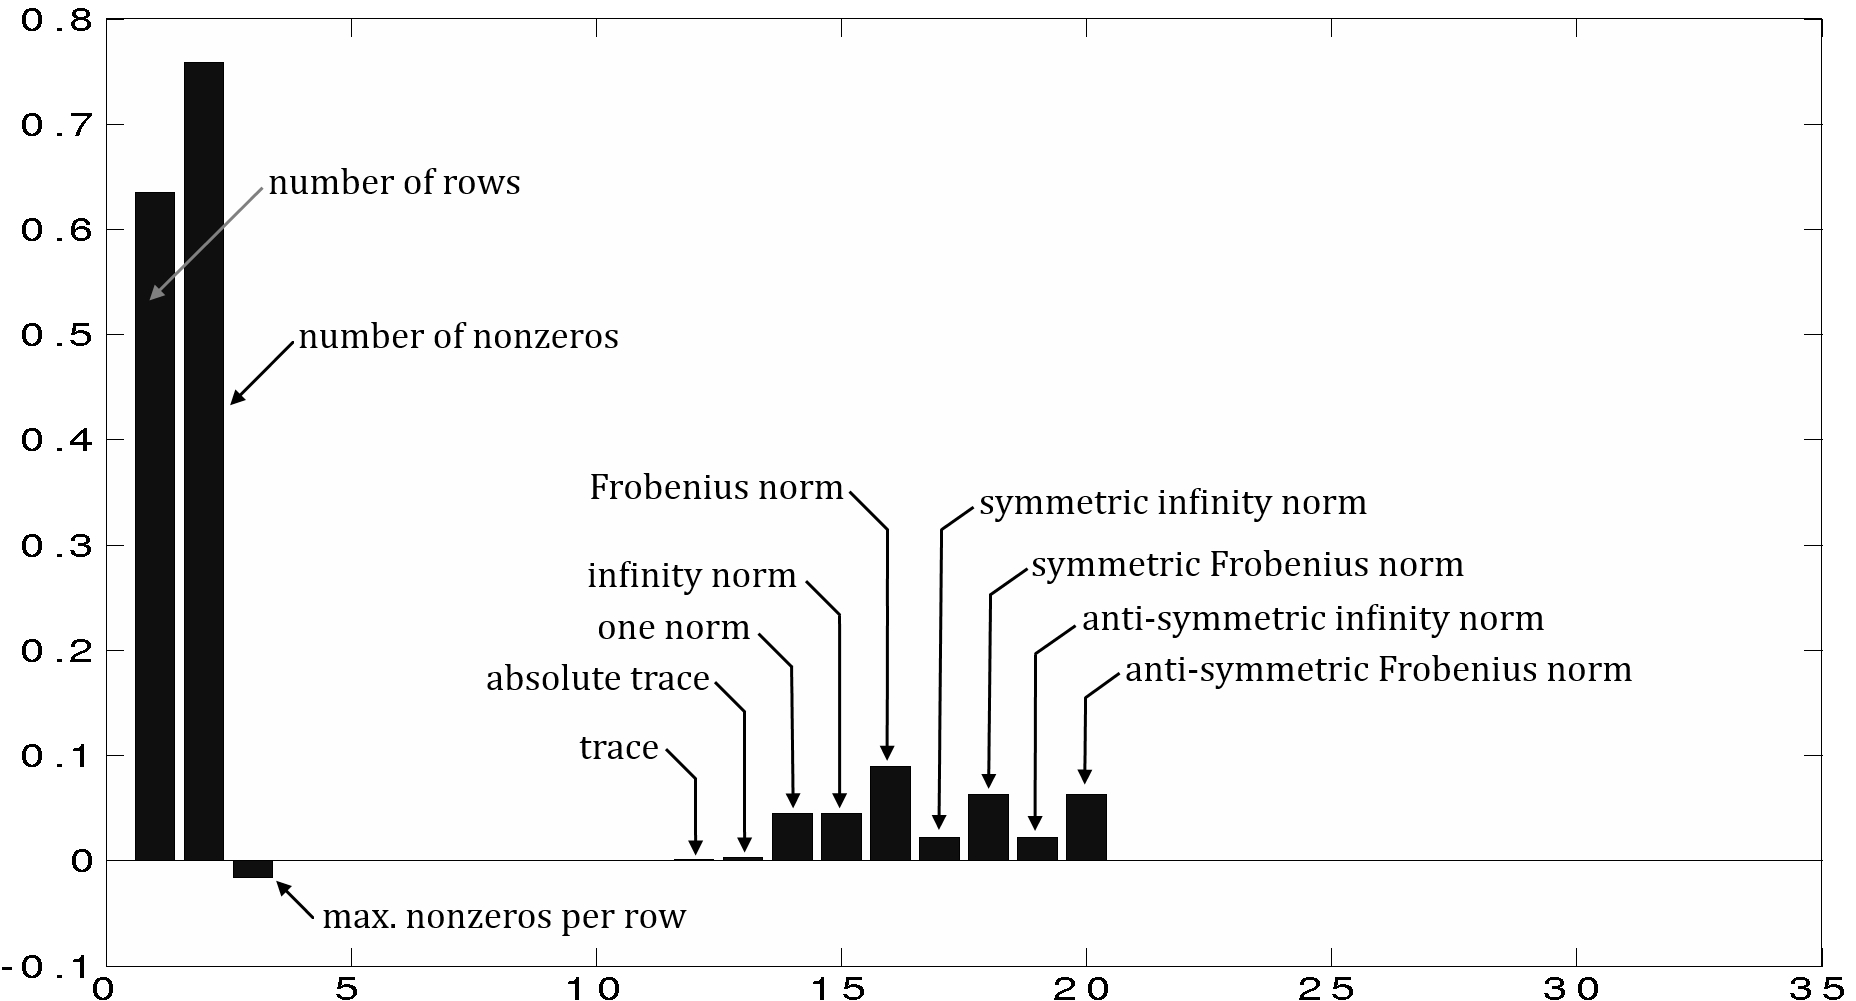
\includegraphics[width=6in]{figs/pc_4l}
  \caption[Fourth principal component.]
   {Fourth principal component.}
\end{figure}

\noindent Based on the PCA results, we decided to use fifteen features out of the thirty features we computed. Table 4.1 shows the reduced feature set and the computation time for each feature for 860 matrices. The computation times were recorded using the hardware and software specified in Table A.1 and A.2.

\begin{table}[H]
 \centering
    \begin{tabular}{| l | c |}
    \hline
    \multicolumn{2}{|c|}{Reduced feature set and computation time} \\
    \hline
    \hline
    Matrix feature & Computation time \\ \hline
    Row variance & 9.90s \\ \hline
    Column variance & 11.47s \\ \hline
    Diagonal variance & 0.16s  \\ \hline
    Number of nonzeros & 1.97s  \\ \hline
    Number of rows & 0.06s \\ \hline
    Frobenius norm & 0.03s  \\ \hline
    Symmetric Frobenius norm & 13.34s  \\ \hline
    Anti-symmetric Frobenius norm & 13.24s  \\ \hline
    One norm &  0.21s \\ \hline
    Infinity norm & 0.07s \\ \hline
    Symmetric infinity norm & 13.33s \\ \hline
    Anti-symmetric infinity norm & 13.44s \\ \hline
    Max. nonzeros per row & 1.95s \\ \hline
    Trace & 0.06s  \\ \hline
    Absolute Trace & 0.15s \\ \hline
    \hline
    Total time & 79.38s \\ \hline
   \end{tabular}
   \caption{Reduced feature set and approximate computation time.}
   \label{tab:featureset}
\end{table}

\section{Dataset}

Our dataset consists of 860 sparse matrices downloaded from the The University of Florida Sparse Matrix Collection \cite{florida}. All the matrices are real and square. The Table 4.2 shows the names and sizes of the matrices that have the minimum and maximum dimension, lowest and highest number of nonzero entries, highest row and column variances. It also shows how many symmetric, unsymmetric, diagonally dominant matrices are there in our dataset.

\begin{table}[H]
 \centering
    \begin{tabular}{| l | c | c |}
    \hline
    \multicolumn{3}{|c|}{Dataset statistics} \\
    \hline
    \hline
    Matrix property & Value & Matrix name \\ \hline
    Minimum dimension & 5\texttimes5 & cage3  \\ \hline
    Maximum dimension & 46772\texttimes46772 & bcsstm39  \\ \hline
    Minimum nonzeros & 19 & cage3  \\ \hline
    Maximum nonzeros & 1137732 & spiral\_E  \\ \hline
    Maximum row variance & 2.02902e36 & mcca  \\ \hline
    Maximum column variance & 1.54208e36 & mcca  \\ \hline
    Numerically symmetric matrices & 211 & n/a \\ \hline
    Numerically unsymmetric matrices & 649 &  n/a  \\ \hline
    Structurally symmetric matrices & 377 & n/a \\ \hline
    Structurally unsymmetric matrices & 483 &  n/a  \\ \hline
    Diagonally dominant matrices & 67 & n/a \\ \hline
    Diagonally nondominant matrices & 793 &  n/a  \\ \hline
   \end{tabular}
   \caption{Various statistics of our dataset.}
   \label{tab:dataset}
\end{table}

\section{Methods used for solving linear systems}

We formed 860 systems of linear equations using the matrices from our dataset and right-hand side vectors with all their entries set to 1. Then we solved the systems using a number of different methods, i.e., various combinations of the following Krylov subspace methods and preconditioners (and also without any preconditioner).
\\
\textbf{Krylov subspace methods:}
\begin{enumerate}
  \item Conjugate Gradient (CG) \cite{cg}
  \item Conjugate Gradient Squared (CGS) \cite{cgs}
  \item BiConjugate Gradient (BICG) \cite{bicg}
  \item BiConjugate Gradient Stabilized (BiCGSTAB) \cite{bicgstab}
  \item Generalized Minimal Residual (GMRES) \cite{gmres}
  \item Flexible Generalized Minimal Residual (FGMRES) \cite{fgmres}
  \item Transpose-Free Quasi-Minimal Residual (TFQMR) \cite{tfqmr}
\end{enumerate}

\noindent \textbf{Preconditioners:}\cite{saadbook}
\begin{enumerate}
  \item ILU(0), ILU(1), ILU(2) (sequential)
  \item Jacobi (sequential), Block Jacobi (parallel)
  \item SOR (sequential and parallel)
  \item ASM (parallel)
\end{enumerate}

\noindent  We observed which methods succeed at solving a particular system and which do not. For each system, we picked the method that converged fastest with solve time $t_{lowest}$  and any other method that converged within the time $1.1 \times t_{lowest}$.

\section{Machine learning techniques}

Machine learning is a branch of artificial intelligence that focuses on building and studying systems that can learn from data. A variety of machine learning techniques has been 
developed for decision making, clustering, pattern recognition, classification and other tasks. Some of the widely used machine learning techniques are decision trees, artificial neural networks, support vector machines, case based reasoning, classification and regression trees \cite{singh}. A research work has been conducted on comparing performances of various machine learning techniques such as Naive Bayes Classifier (NB), Support Vector Machine (SVM), Alternating Decision Tree (ADT), Decision Stump (DS), Instance-based Learning (IB1, IBk), for selecting linear solvers using matrix features similar to ours \cite{brice}. The accuracies of all the machine learning techniques from that research work is shown in Figure 4.16 (results for symmetric matrices) and 4.17 (results for unsymmetric matrices).

\begin{figure}[H]\label{brice_1}
  \centering
  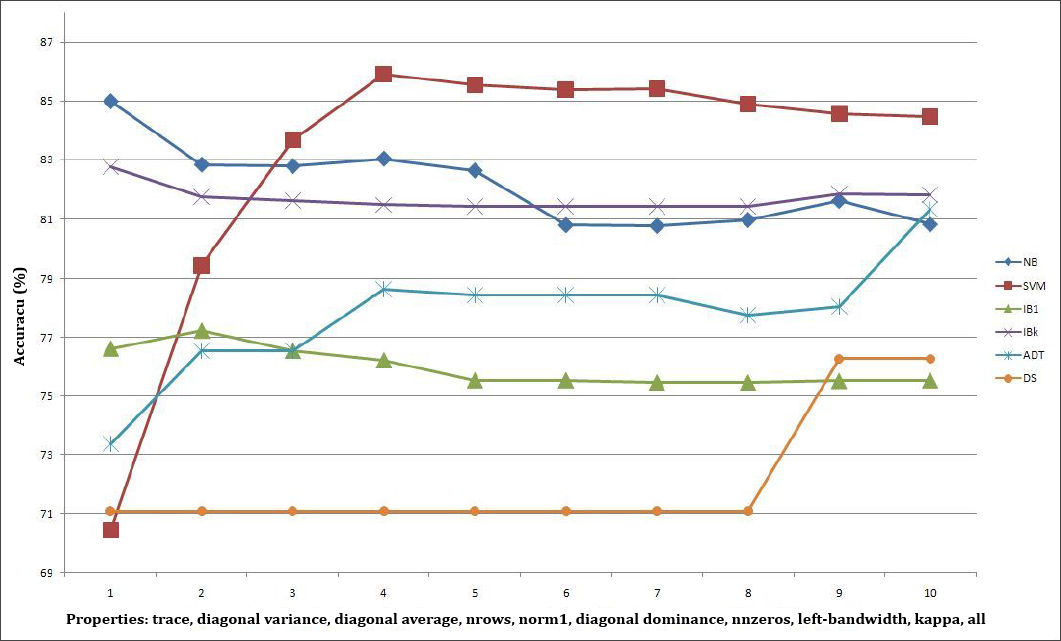
\includegraphics[width=6in]{figs/brice_1}
  \caption[Accuracy of classifiers for symmetric matrices.]
   {Accuracy of classifiers for symmetric matrices \cite{singh}.}
\end{figure}

\begin{figure}[H]\label{brice_2}
  \centering
  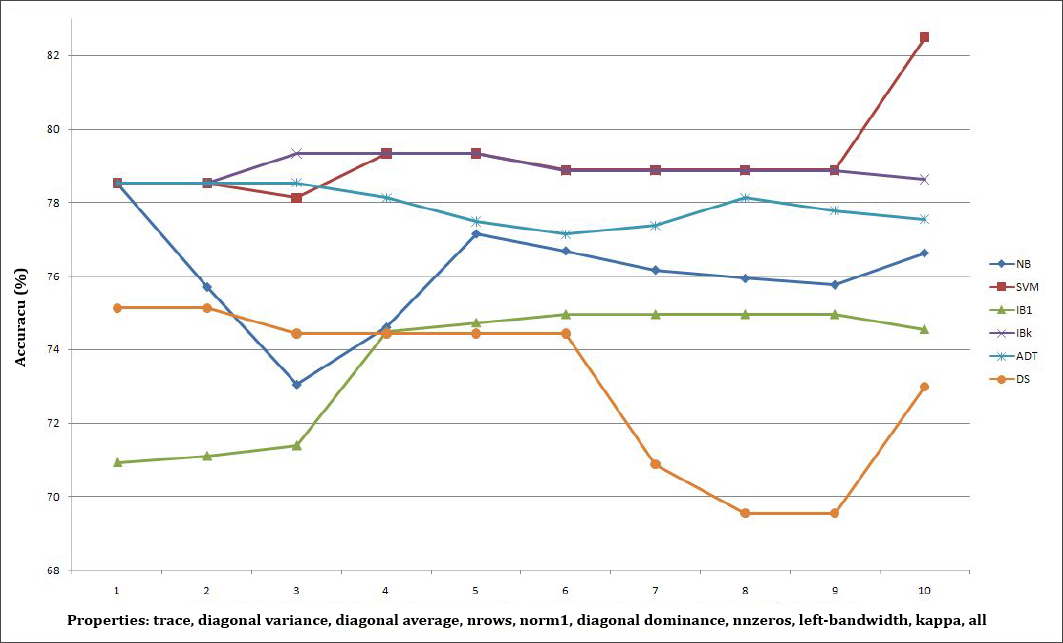
\includegraphics[width=6in]{figs/brice_2}
  \caption[Accuracy of classifiers for unsymmetric matrices.]
   {Accuracy of classifiers for unsymmetric matrices \cite{singh}.}
\end{figure}

\noindent We can see that SVM achieves the highest accuracies for both symmetric and unsymmetric matrices. Based on these results, we decided to use SVM for our purposes.

\subsection{Support Vector Machine (SVM)} Support Vector Machine is an machine learning approach where the SVM takes a set of training data consisting of observations from two classes, then tries to separate the observations from the two classes and predicts, for each input, which of the two possible classes forms the output. Consider $k$ training data points $D_{T}$, where each input \textbf{x}$_{i}$ is a point on an $n$-dimensional space and belongs two either of the two classes $y_{i} = 1$ or $-1$, that is,\begin{center} $D_{T} = \{($\textbf{x}$_{i},y_{i})\}$ where $ i = 1...k$,  $y_{i} \in \{-1,1\}, $ \textbf{x} $ \in \Re^{n}$.\end{center} In our case, we assume the data points are linearly separable. So we can draw a line on a graph of $x_{1}$ vs $x_{2}$ and separate the two classes when $n=2$. If $n>2$ then we draw a hyperplane on graphs of $x_{1},x_{2}...x_{n}$ to separate the points. This hyperplane is defined by \textbf{w}$\cdot$\textbf{x} $+$ $b = 0$, where $\cdot$ denotes the dot product, \textbf{w} is normal to the hyperplane and $b$ is a scalar value. $\frac{b}{||w||}$ is the offset of the hyperplane from the origin along \textbf{w}. Support Vectors are the points that are closest to the separating hyperplane. The goal of the SVM is to orientate this hyperplane in such a way that it is as far away as possible from the closest members of both classes. We then select \textbf{w} and $b$ so that the training data points can be expressed by \textbf{x}$_{i}\cdot$\textbf{w} $+$ $b \geq 1$ for $y_{i} = 1$ and \textbf{x}$_{i}\cdot$\textbf{w} $+$ $b \leq -1$ for $y_{i} = -1.$  Figure 4.18 shows a linear hyperplane with support vectors circled.

\begin{figure}[H]\label{svm}
  \centering
  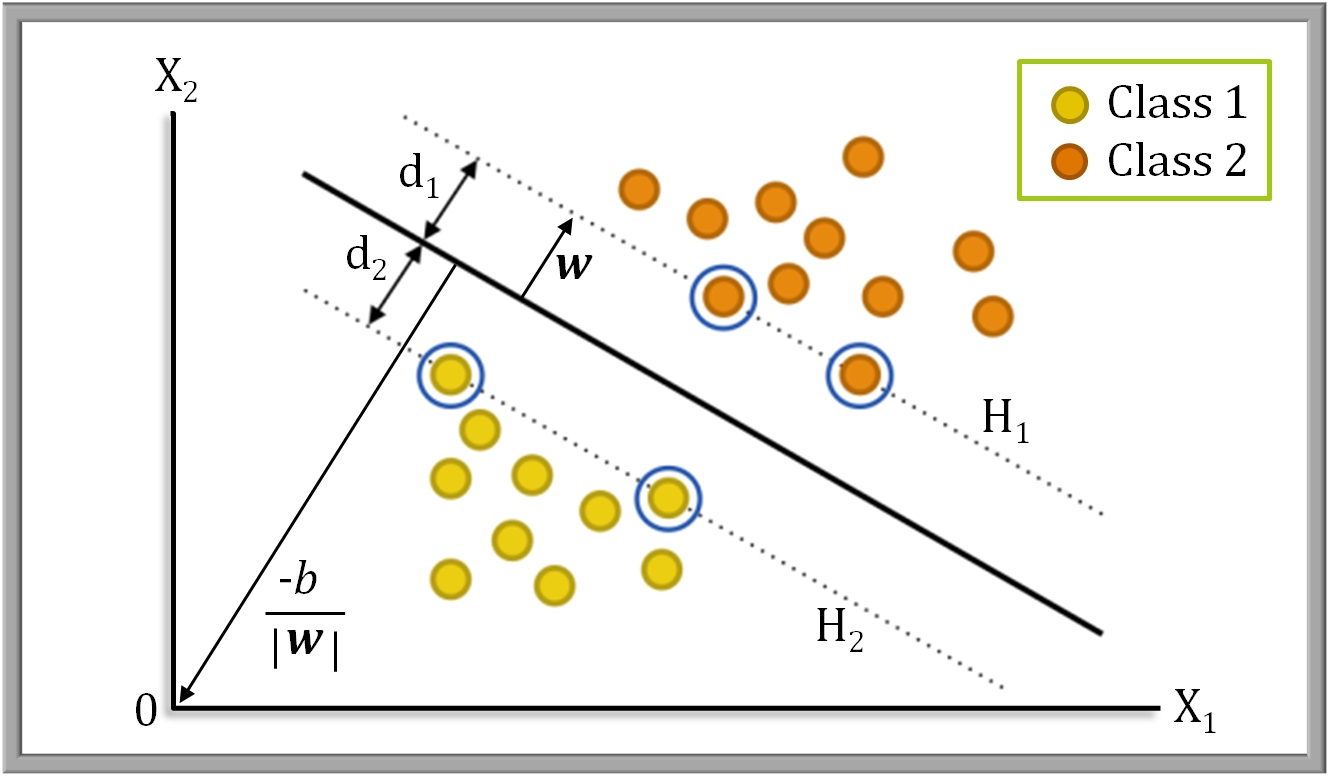
\includegraphics[width=4.5in]{figs/svm}
  \caption[Options for users who choose not to upload their matrix.]
   {Support Vector Machine, hyperplane separating members of two classes.}
\end{figure}

We used the SVM classifier from Matlab's Bioinformatics Toolbox. For preparing the training data point for a matrix, we formed a vector containing fifteen features of that matrix and a scalar value indicating which KSP and PC were used to solve the linear system. If a certain pair of KSP and PC gives the fastest solution in $t_{lowest}$ seconds or a near fastest solution within $1.1 \times t_{lowest}$ seconds, then the data point belongs to Class 1. If a pair of KSP and PC does not give the fastest or a near fastest solution, then the data point belongs to Class 2. 

For the sequential case, we solved each matrix in our dataset of 860 matrices sequentially with forty-one different methods (i.e., pairs of KSP and PC) giving us $860 \times 41 = 35260$ data points, where each one is a 16-dimensional vector. For the parallel case, we solved 860 matrices using four processes with twenty-seven different methods. The number of methods used for the parallel case is lower than the sequential case because we used six different preconditioning techniques for the sequential case but only four preconditioning techniques for the parallel case. The number of data points for the parallel case is $860 \times 27 = 23220$ and each data point is a 16-dimensional vector.

\section{Test results}

We used k-fold cross-validation \cite{provost} with $k=10$ for calculating the accuracy of our system. $k$-fold cross-validation is a method for estimating the accuracy of a model. The data set is partitioned into $k$ subsets which are known as `folds'. In each iteration of training and testing, one of the $k$ subsets is used as the test set and the rest of the $k-1$ subsets are combined and used as the training set. The error from all $k$ iterations are averaged. Every sample in the dataset gets used for testing exactly one time and gets used for training $k-1$ times.

We present our results in the form of confusion matrices \cite{provost}. A confusion matrix shows the actual and predicted classifications. Table 4.3 shows the SVM classification results for the sequential case and Table 4.4 shows the classification results for the parallel case.

\begin{table}[H]
 \centering
\begin{tabular}{cc|c|c|c}
\cline{3-4}
& & \multicolumn{2}{ c| }{Actual} \\ \cline{3-4}
& & Class 1 & Class 2   \\ \cline{1-4}
\multicolumn{1}{ |c| }{\multirow{2}{*}{Predicted} } &
\multicolumn{1}{ |c| }{Class 1} & a = 1031 & b = 4821        \\ \cline{2-4}
\multicolumn{1}{ |c  }{}                        &
\multicolumn{1}{ |c| }{Class 2} & c = 322 & d = 29086       \\ \cline{1-4}

\end{tabular}
\caption{SVM classification results for the sequential case.}
\end{table}

\noindent The entries in the confusion matrix have the following meaning:
\begin{itemize}
 \item $a =$ number of correct predictions that an instance belongs to Class 1,
 \item $b =$ number of incorrect predictions that an instance belongs to Class 1,
 \item $c =$ number of incorrect predictions that an instance is belongs to Class 2,
 \item $d =$ number of correct predictions that an instance belongs to Class 2.
\end{itemize}

\begin{table}[H]
 \centering
\begin{tabular}{cc|c|c|c}
\cline{3-4}
& & \multicolumn{2}{ c| }{Actual} \\ \cline{3-4}
& & Class 1 & Class 2   \\ \cline{1-4}
\multicolumn{1}{ |c| }{\multirow{2}{*}{Predicted} } &
\multicolumn{1}{ |c| }{Class 1} & a = 175 & b = 3400        \\ \cline{2-4}
\multicolumn{1}{ |c  }{}                        &
\multicolumn{1}{ |c| }{Class 2} & c = 792 & d = 18853       \\ \cline{1-4}

\end{tabular}
\caption{SVM classification results for the parallel case.}
\end{table}


\noindent The accuracy $Ac$ is the proportion of the total number of predictions that were correct. It is evaluated using the equation:

\begin{equation}
  Ac = \frac{a+d}{a+b+c+d}
\end{equation}

\noindent Determined using Equation 4.3, the average accuracy of the classifier for the sequential case is 85.41\% and parallel case is 81.95\%.

\subsection{How Lighthouse uses SVM}

After Lighthouse receives the matrix file and user's choice indicating whether the user wants to run the program sequentially or in parallel, it executes the following steps.

\begin{enumerate}
\item Lighthouse extracts the matrix features.
\item Lighthouse creates a set of vectors (41 for the sequential case, 27 for the parallel case). Each vector is created by inserting the matrix features as its entries and then an additional entry is inserted that indicates a specific method (i.e., a KSP and a PC). Thus, the last entry of each vector is unique but the remaining entries are the same for all vectors.
\item Lighthouse then uses the SVM classifier on each of the vectors.
\item If any of the vectors are classified as a Class 1 vector, Lighthouse notes down the method indicated by the last entry of that vector. If multiple vectors are classified as Class 1 vectors, Lighthouse notes down all the methods. If none of the vectors are classified as a Class 1 vector, Lighthouse notes down that none of the methods are likely to produce a good solution.
\item Lighthouse then provides the user with a PETSc program for solving the linear system, a makefile for compiling the program, a text file with instructions and another text file that suggests one or more methods that are likely to give a good solution. If none of the methods are predicted to give a good solution, Lighthouse notifies the user through the web user interface instead of providing them with any file.
\end{enumerate}

\subsection{Training and testing time}

Table 4.5 shows the average training and testing times for the sequential and parallel cases. The computation times were collected using the hardware and software specified in Table A.1 and A.2.

\begin{table}[H]
 \centering
    \begin{tabular}{| l | c | c | c | c |}
    \hline
    \multicolumn{5}{|c|}{Classifier training and testing time} \\
    \hline
    \hline
     & Training time & Training instances & Testing time & Test instances\\ \hline
    Sequential case & 349.10s & 31734 & 2.85s & 3526\\ \hline
    Parallel case & 66.75s & 20898 & 0.61s & 2322\\ \hline
   \end{tabular}
   \caption{Classifier training and testing times.}
   \label{tab:tnttime}
\end{table}
